\section{Feedback (informally)}
\subsection{}

\begin{frame}\mccz
\frametitleTC{Feedback and its magic}
\myPause
 \begin{columns}
  \column[T]{0.45\textwidth}
   \only<2->{\centering
\includegraphics[height=6cm]{./Unit-02/img/Feedback-TheMagic_cc0.jpg}}\myPause%
  \column[T]{0.55\textwidth}
   \begin{itemize}[<+-| alert@+>]
   \item If PROPERLY used, feedback can
         \begin{itemize}[<+-| alert@+>]
         \item \vspace{2mm}counteract model errors\\
                and uncertainties,
         \item \vspace{2mm}reject a disturbance\\
                without the need\\
                for its measurement,
         \item \vspace{2mm}stabilise an unstable\\
               or ``runaway'' system.
         \end{itemize}
   \item \vspace{4mm}Let us see.
   \end{itemize}
 \end{columns}
\end{frame}

\begin{frame}
\frametitleTC{Feedback to counteract model errors/uncertainty and disturbances}
\framesubtitleTC{(to introduce this idea we do not use dynamic systems for simplicity)}
\myPause
 \begin{itemize}[<+-| alert@+>]
 \item \vspace{-8mm}Consider a controlled system such that the outcome $O$ depends on the control action $A$ and
       the disturbance $D$ as \textcolor{magenta}{$O=0.5(A+D)$.}
 \item If we want to use open-loop control and to make $O$ equal a reference $R$, we must solve for $A$ the equation
       $0.5(A+D)=R$, whence the control law \DG{$A=2R-D$.}
 \item Let us verify with some numbers:
 \item[] \begin{center}
          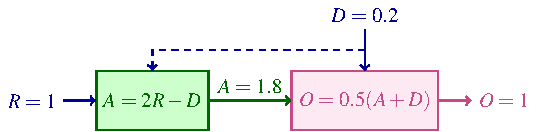
\includegraphics[width=0.60\columnwidth]{./Unit-02/img/Taxonomy-OpenLoop-Example-FullKnowledge.pdf}
          \hspace{6mm}
\includegraphics[height=1.5cm]{./Unit-02/img/smile.png}
         \end{center}
 \end{itemize}
\end{frame}

\begin{frame}
\frametitleTC{Feedback to counteract model errors/uncertainty and disturbances}
\myPause
 \begin{itemize}[<+-| alert@+>]
 \item But what if we assume \textcolor{magenta}{$O=0.5(A+D)$} while the true system is
       \textcolor{magenta}{ $O=\mathbf{0.6}(A+D)$}?
 \item If we use the nominal control law \DG{$A=2D-R$} on the true system, we get the following:
 \item[] \begin{center}
          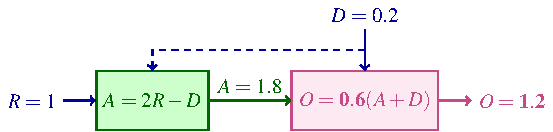
\includegraphics[width=0.65\columnwidth]{./Unit-02/img/Taxonomy-OpenLoop-Example-PartialKnowledge.pdf}
          \hspace{6mm}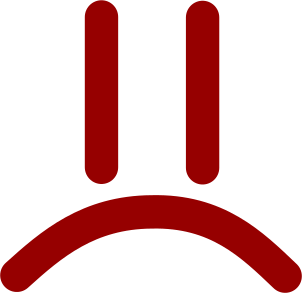
\includegraphics[height=1.5cm]{./Unit-02/img/frown.png}
         \end{center}
 \item \vfill H\'{e}las, 20\% error on a model parameter (0.6 instead of 0.5)\\
       $\Rightarrow$ 20\% error of $O$ wrt $R$.
 \item Open-loop control cannot counteract model errors.
 \item Let us try with feedback.
 \end{itemize}
\end{frame}

\begin{frame}
\frametitleTC{Feedback to counteract model errors/uncertainty and disturbances}
\myPause
 \begin{itemize}[<+-| alert@+>]
 \item \underline{EXAMPLE} feedback scheme with \TC{proportional} control (action $A$ proportional\\
       to the \TC{error} $R-O$); note that we do not compensate the disturbance:
 \item[] \begin{center}
          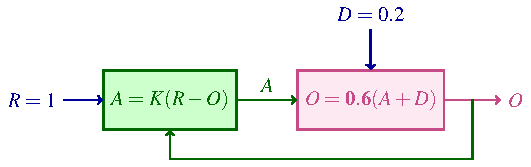
\includegraphics[width=0.60\columnwidth]{./Unit-02/img/Taxonomy-ClosedLoop-Example.pdf}
         \end{center}
 \item Joining the system and controller equations, for $O$ we get
       \begin{displaymath}
        \begin{array}{rcl}
         \left\{\begin{array}{rl}
          A &= K(R-O) \\
          O &= 0.6(A+D)
         \end{array}\right. &
         \Rightarrow &
          O = \frac{3K}{3K+5}R+\frac{3}{3K+5}D
         \end{array}
        \end{displaymath}
 \item Apparently, as $K \rightarrow \infty$, $O \rightarrow R$ $\forall D$.
 \item \vfill Yes, feedback can counteract model errors and disturbances;
 \item possible drawbacks on stability (improper use of feedback) later on. 
 \end{itemize}
\end{frame}

\begin{frame}
\frametitleTC{Studying the stability of a system}
\framesubtitleTC{adopting here a \underline{very} informal attitude, where ``stable'' means ``left alone, does not
                 run amok''}
\myPause
 \begin{itemize}[<+-| alert@+>]
 \item Let us take our system, initialise $y(0)$ to $y_0$, let $u(k)=0$ $\forall k$ so that
       \begin{displaymath}
        y(k) = ay(k-1),
       \end{displaymath}
       and see what happens.
 \item \vfill Case 1: $|a|<1$, for example 0.5 or -0.5.\\
 \item[] For $k=0,1,2,\ldots$, we have respectively the $y$ sequences
       \begin{displaymath}
        \begin{matrix*}[r]
          y_0, &  0.5y_0, & 0.25y_0, &  0.125y_0, \ldots \\
          y_0, & -0.5y_0, & 0.25y_0, & -0.125y_0, \ldots
        \end{matrix*}
       \end{displaymath}       
 \item[] For $k\rightarrow\infty$ the system's \TC{free motion} (no input) converges to zero\\
         $\Rightarrow$ we say the system is \TC{asymptotically stable.}      
 \end{itemize}
\end{frame}

\begin{frame}
\frametitleTC{Studying the stability of a system}
\myPause
 \begin{itemize}[<+-| alert@+>]
 \item Case 2: $|a|=1$, i.e., $a=\pm 1$.\\
 \item[] For $k=0,1,2,\ldots$, we have respectively the $y$ sequences
       \begin{displaymath}
        \begin{matrix*}[r]
          y_0, &  y_0, & y_0, &  y_0, \ldots \\
          y_0, & -y_0, & y_0, & -y_0, \ldots
        \end{matrix*}
       \end{displaymath}       
 \item[] For $k\rightarrow\infty$ the free motion neither converges to zero nor diverges\\
         $\Rightarrow$ we say the system is \TC{stable}, but not asymptotically.
 \item \vfill Case 3: $|a|>1$, for example 2 or -2.\\
 \item[] For $k=0,1,2,\ldots$, we have respectively the $y$ sequences
       \begin{displaymath}
        \begin{matrix*}[r]
          y_0, &  2y_0, & 4y_0, &  8y_0, \ldots \\
          y_0, & -2y_0, & 4y_0, & -8y_0, \ldots
        \end{matrix*}
       \end{displaymath}
 \item[] For $k\rightarrow\infty$ the free motion diverges (except for the one case $y_0=0$)\\
         $\Rightarrow$ we say the system is \TC{unstable.} 
 \end{itemize}
\end{frame}


\begin{frame}
\frametitleTC{Stabilising a system by means of feedback}
\myPause
 \begin{itemize}[<+-| alert@+>]
 \item Take an unstable system:
       \begin{displaymath}
        y(k) = ay(k-1)+u(k-1), \qquad a=2.
       \end{displaymath}
 \item Feed $y$ back to $u$ proportionally, i.e., set $u(k) = Qy(k)$.
 \item Doing so we have the closed-loop system
       \begin{displaymath}
        y(k) = 2y(k-1)+Qy(k-1) = (2+Q)y(k-1)
       \end{displaymath}
       and if we chose $Q$ so that $|2+Q|<1$, this is asymptotically stable.
 \end{itemize}
\end{frame}

\begin{frame}
\frametitleTC{Stabilising a system by means of feedback}
\framesubtitleTC{and once again, tolerating model errors/uncertainties}
\myPause
 \begin{itemize}[<+-| alert@+>]
 \item Note that feedback control is also naturally \TC{robust} (for the moment,\\
       think of this as ``resilient to model errors'').
 \item For example, take $Q=-1.5$ so that $2+Q=0.5$.
 \item In this case the closed loop is asymptotically stable not only for $a=2$,\\
       but $\forall a$ s.t. $|a+Q|=|a-1.5|<1$, i.e., for $0.5<a<2.5$.
 \item \vspace{4mm} Summing up, with feedback we can impose stability even if we do not know\\
       the system (here, parameter $a$) precisely...
 \item[]\vspace{-1mm} ...but for the very same reasons, we might also \emph{destroy} stability.
 \item Feedback is a powerful weapon, use with care.
 \item \vfill And now, let us re-address feedback and dynamic systems\\
       with a formal attitude (soon focusing on the DT LTI case).
 \end{itemize}
\end{frame}


